\section{Benchmarks}\label{sec:benchmarks}
\subsection{Parameters and Security Estimations}
The dimension of the ring $\ring$ is fixed to $n=512$.
The constraints to derive workable parameters are summarized in Table \ref{tab:constraints}.
To find concrete parameters, a script\footnote{\label{fn:github}\url{https://github.com/GottfriedHerold/Chipmunk}} was used to enumerate possible parameters subject to these constraints and additionally subject to leading to hard ring-SIS problems and allowing for efficient NTT evaluation.
For any choice of $\secpar\in\{112,128\}$, $\rho\in\NN$, and $\tau\in\NN$ this script then finds the parameter set that allow for the smallest possible signature size.
For convenience, the results of running the script for a range of reasonable inputs are reproduced in \autoref{tab:param} in the appendix.
\begin{table}
  \centering
  \begin{tabular}{@{\makebox[3em][r]{\rownumber\space}} l@{\hspace{3em}}rl}
  \toprule
   \multicolumn{1}{@{\makebox[3em][r]{\#\space}} c}{Source}&\multicolumn{2}{c}{Constraint}\\
  \midrule
   \autoref{lem:hvcprobhom}&$\bagg \geq$&$ \eta\sqrt{2\alpha_w\rho(\epsilon + 1 + \log_2 n + \log_2(2\tau \lceil\log_{2\eta+1}q\rceil + \xi\lceil\log_{2\eta+1}q'\rceil))\cdot\ln2}$\\
   \autoref{lem:kots_correct}& $\beta_\sigma \geq$&$ 4\varphi\alpha_H\sqrt{\tfrac{1}{2}\alpha_w\rho(\varepsilon+1+\log_2n\gamma)\cdot\ln2}$\\
   \autoref{lem:kots_sis}&$\abs{\tern_{\alpha_H}} \geq$&$ 2^{2\secpar}$\\
   \autoref{lem:keyhidden}& $\gamma\geq$&$((3\secpar+\delta)/n+\log_2q)\log^{-1}_2(\varphi+\tfrac{1}{2})$\\
   \autoref{lem:keyhidden}& $\abs{\tern_{\alpha_H}} \leq$&$ 2^{2\secpar + \delta}$\\
   \autoref{lem:nilssupportivechildsupport}&$q'>$&$ 16 \alpha_w \alpha_H\varphi$\\
   \autoref{lem:msigaggcorrect}&$\chi \geq$ &$\secpar/(\varepsilon-1)$\\
   \autoref{lem:msigunf}&$\abs{\tern_{\alpha_w}} \geq$&$2^\secpar$
  %\bottomrule
  \end{tabular}
  \caption{The constraints a set of Chipmunk parameters needs to satisfy to ensure that the proofs are applicable. The parameters additionally need to be chose such that the associated Ring-SIS problems are hard.}\label{tab:constraints}
  \end{table}
  
We briefly explain how the constraints implemented in the scripts.
First, to ensure security of Chipmunk, the specific ring-SIS problems in Lemma \ref{lem:hvcprobhom} and \ref{lem:kots_correct} need to be hard.
We use the same approach to derive the security of the parameters as was used in Squirrel \cite{CCS:FleSimZha22}.
We adopt the so-called \enquote{realistic model} from \cite{USENIX:ADPS16}.
For a BKZ of block size $\beta$, the cost in this model is estimated by
$2^{0.292\beta+16.4+\log(\#\texttt{SVP calls})}$. 
The LWE-estimator \cite{DBLP:journals/jmc/AlbrechtPS15}
shows that for a root Hermite factor of $1.005$ we expect a block size of 286, which yields $112$ bits of security under the above model.
Similarly, a root Hermite factor of $1.004$ yields $128$ bits of security.

Then, on the output of the hash of the message, we need it to be large enough
to be security against meet-in-the-middle type of attacks; 
in the meantime, for the security proof,
we also need to customize $\tern_{\alpha_H}$, such that, 
for a given public parameter $\vec{a}$, a fixed hash digest in $\tern_{\alpha_H}$,
and a signature $\vec{\sigma}$ for the one time signature scheme,
there exists at least two short $(\vec{s}_0, \vec{s}_1)$ with overwhelming probability.

Lastly, we also require every randomizer to be unguessable, and therefore $\abs{\tern_{\alpha_w}} \geq 2^\secpar$.

\subsection{Implementations}
Chipmunk was implemented in Rust. The source code, as well as the scripts for parameter derivation are released to the open domain\footnoteref{fn:github}.

\subsubsection{Comparisons}\label{ss:comparison}
Chipmunk can be reasonably compared with two points of reference:
the trivial solution, i.e., storing a list of $\rho$ Falcon signatures and using
Squirrel \cite{CCS:FleSimZha22}, the previous state-of-the-art.
The data for Chipmunk and Squirrel are collected over a same benchmark platform, an AMD 5900x with 24 threads and 32 Gigabytes of memory.
The data for Falcon-512 is collected from the official website\footnote{\url{https://falcon-sign.info/}}.
All three candidates are instantiated to yield $112$ bits security.

The comparison with the trivial solution is quite straightforward.
Since its signature size grows linearly with the number of signers,
Chipmunk can easily improve by a couple of orders of magnitudes when the number of signers increases.
Also note that the signing speed of Chipmunk is of the same order of magnitude as Falcon-512.

In terms of Squirrel, we see that for both $\rho = 1024$ and $\rho = 8192$, our scheme is better in all metrics.
In particular, there are two main obstacles that would prevent Squirrel from being widely deployable, the key generation time and the signature size.
The benchmarks show that key generation time is improved by a factor of $9$ on the same platform.
The aggregated signature size is reduced by a factor of $4.8$.
\bgroup
\setlength{\tabcolsep}{0.5em}
\renewcommand{\arraystretch}{1.1}
\begin{table}\centering
  \begin{tabular}{clccccc}
    \# signers      &                 & Falcon      & Squirrel  & Chipmunk  & Imp. Falcon & Imp. Squirrel \\\toprule
    \multirow{2}{*}{} 
                    & Key Generation  & 8.6 ms      & 4 min     & 26.5 sec  &     -       & 9.0$\times$ \\%\cline{2-7}
                    & Signing         & 0.17 ms     & 2.1 ms    & 0.4 ms    &     -       & 5.2$\times$ \\%\cline{2-7}
                    &Fresh Sig. Size  & 666 Bytes   & 45 KB     & 32 KB     &     -       & 1.4$\times$ \\\midrule
    \multirow{3}{*}{1024}                
                    &Aggregation      & -           & 1.2 sec   & 0.55 sec  &     -       & 2.2$\times$ \\%\cline{2-7}
                    &Batch Verification    
                                      & 36.7 ms     & 19.5 ms   & 7.2 ms    & 5.1$\times$ & 2.7$\times$ \\%\cline{2-7}
                    
                    &Agg. Sig. size   & 682 KB      & 572 KB    & 142 KB    & 4.8$\times$ & 4.0$\times$ \\\midrule
    \multirow{3}{*}{8192}                
                    &Aggregation      & -           & 9.6 sec   & 4.3 sec   &     -       & 2.2$\times$ \\%\cline{2-7}
                    &Batch Verification    
                                      & 294 ms      & 53  ms    &  47 ms    & 6.2$\times$ & 1.1$\times$ \\%\cline{2-7}
                    &Agg. Sig. size   & 5.5 MB      & 762 KB    & 160 KB    & 340$\times$ & 4.8$\times$\\ \bottomrule
  \end{tabular}
  \caption{Comparison of Chipmunk, Squirrel, and a trivial solution based on concatenating``\# signers'' many Falcon-512 signatures. Squirrel and Chipmunk are instantiated with $\secpar = 112$ and $\tau=21$.}

\end{table}

\subsubsection{Practical Performance}
To show that Chipmunk is practical we take a closer look at the key generation time and the aggregated signature size.

We conducted a benchmark over a typical server that is equipped with an AMD 7773x with
64 cores and 1 Terabytes of memory.
The results are summarized in Table \ref{tab:bench_results}.
Notice that this platform is different from that of \autoref{ss:comparison},
and more accurately simulates the real world node runners for blockchains.

\begin{table}[t]\centering
  \begin{tabular}{ccccccc}
      Tree Height         & Key Generation            & Online Signing\footnotemark        
      & $\#$ Signers  
                                                                                            &  Aggregation & Verification  & Agg. Sig. Size  \\ \toprule
      \multirow{2}{*}{21} & \multirow{2}{*}{7.4 sec}  & \multirow{2}{*}{0.40 ms}  & 1024    &   491 ms     &  7.3 ms       & 142 KB     \\%\cline{4-7}
                          &                           &                           & 8192    &   3.5 sec    &  42.3 ms      & 160 KB     \\\hline

      \multirow{2}{*}{24} & \multirow{2}{*}{1 min}    & \multirow{2}{*}{0.44 ms}  & 1024    &   492 ms     &  7.5 ms       & 160 KB     \\%\cline{4-7}
                          &                           &                           & 8192    &   3.8 sec    &  42.1 ms      & 180 KB     \\\hline

      \multirow{2}{*}{26} & \multirow{2}{*}{  4 min}  & \multirow{2}{*}{0.44 ms}  & 1024    &   518 ms     &  7.1 ms       & 172 KB     \\%\cline{4-7}
                          &                           &                           & 8192    &   4.0 sec    &  42.9 ms      & 194 KB     \\\bottomrule

  \end{tabular}\\
  \caption{Benchmark results}
  \label{tab:bench_results}
\end{table}
\egroup
\footnotetext{Similar to Squirrel~\cite{CCS:FleSimZha22}, Chipmunk is an online-offline signature scheme, since the opening of the vector commitment can be computed ahead of time without knowing the message to be signed.
This means that online signing only consists of computing the one-time signature.
The secret key of Chipmunk is a large tree, which can be rederived from a pseudorandom seed whenever needed.
This is computationally quite expensive, but asigner can trade storage size against offline signing speed by caching the top layers of the tree.
The reported times for signing correspond to the \emph{online} signing time.
}
% \end{table}
% \subsection{Micro Benchmarks}
As can be seen in \autoref{fig:keygen}, the key generation time scales linearly in the height of the tree as expected.
For the largest parameter set with $\tau = 26$ we can generate a keypair in just 4 minutes, significantly improving over the 2 hour key generation time of Squirrel.
Such a key would be sufficient for 21 years of usage assuming each block takes 10 seconds to finalize as in the case of Ethereum. 
We conclude that the key generation time is no longer a bottleneck for practical deployment.
\begin{figure}[H] 
  \centering
  \begin{subfigure}[b]
  {0.49\textwidth}    \centering
  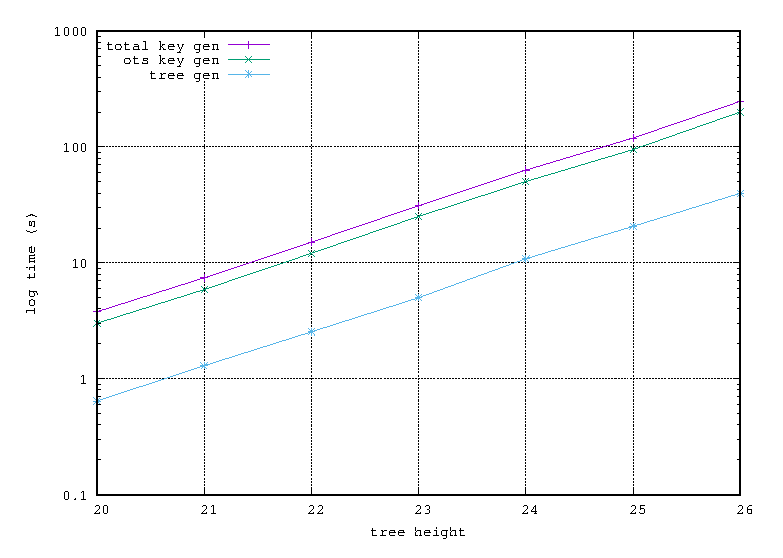
\includegraphics[trim={1mm 0 4mm 0},clip,width=\textwidth]{figures/key_gen.eps}\\
  \caption{Chipmunk key generations time.}
  \label{fig:keygen}
  \end{subfigure}
\begin{subfigure}[b]{0.49\textwidth}    \centering
  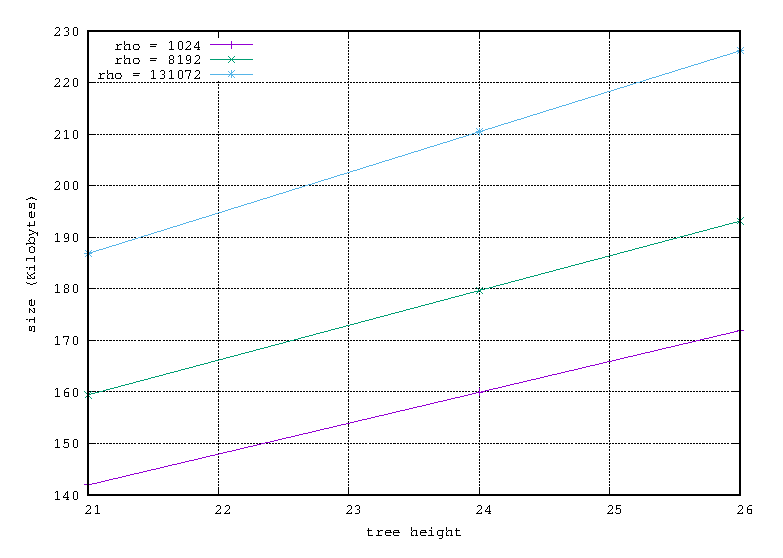
\includegraphics[trim={1mm 0 4mm 0},clip,width=\textwidth]{figures/sig_size.eps}\\
  \caption{Chipmunk aggregated signature size}
  \label{fig:sigize}
  \end{subfigure}
  \caption{Plots showing the scaling characteristics of the key generation time and aggregated signature size of Chipmunk.}
\end{figure}

In terms of the signature size, we'll take as an examle the parameter set with $\tau=21$ and $\rho=1024$.
Here an aggregated signature is of size $142$ Kilobytes, consists of 
\begin{itemize}
  \item the aggregated path to the root and its adjacent nodes, i.e., $2\tau\lceil\log_{2\eta+1}q\rceil$ polynomials in $\ring$ with an infinity norm bound $\bagg <2^{15}$.
  This adds up to $126$ Kilobytes.
  \item the aggregation of decomposed public keys for the one time signature scheme, i.e., $2\lceil\log_{2\eta+1}q'\rceil$ polynomials in $\ring$ with norm bound $\bagg < 2^{15}$, or $8$ Kilobytes 
  \item the aggregated one time signature, i.e., $\gamma$ polynomials in $\mathcal{R}$ with norm bound $\beta_\sigma < 2^{20}$, or $8$ Kilobytes.
\end{itemize}
This almost fits inside a single ethereum block whose peak size is around 130 Kilobytes to date\footnote{\url{https://etherscan.io/chart/blocksize}}.
